\begin{abstract}
Neural network applications of ever-growing size and their adaptations for a growing number of different and sometimes less powerful devices necessitate pruning, the reduction in network size through the removal of superfluous substructures. The term pruning usually implies that the network in question has absolved training until convergence; techniques for a-priori reductions are generally referred to as network architecture search.\\
While most pruning techniques retain the weights of the trained network, in their paper "The Lottery Ticket Hypothesis: Finding Sparse, Trainable Neural Networks," J. Frankle and M. Carbin present a novel technique which resets the weights of the pruned network to their pre-training values.\\
\\
The primary aim of this thesis is to extend their work and research whether the presented algorithm can provide competitive pruning on different datasets, specifically in the field of natural language processing. As the reset to initial values leaves said algorithm similar to a network architecture search method, the pruning can be interpreted as a search dependant on the weights of the trained network. This work also studies how this search develops in quality over the amount of training provided beforehand.\\
\\
In pursuit of these two goals, we developed a framework through which we implemented four experiments. The first and second experiments aim to confirm the validity of the codebase. Subsequently, the third one intents to establish an argument for the usage of the pruning method in the field of natural language processing. With the last experiment, we plan to provide explorative data to inform further study on the emergence of actionable experience in the values of a network.\\
\\
While the first two experiments fail to reproduce the results of J. Frankle and M. Carbin, one of them prunes its associated networks up to the scale contemporary technique, namely a size reduction of 90 percent with little loss in accuracy. Additionally, the third result conforms with their definition of a lottery ticket, achieving the same or even better quality measure, up to the same degree of compression. Finally, the data of the exploratory experiment show low legibility due to the erratic results of single prunings. Nonetheless, none of the early pruning trials achieve the same level of accuracy displayed by our previous experiment, even if the latter trials prune as late as epoch 10, an amount of training for which the full network already converges. These results suggest that, during the pruning iterations,  the pruning algorithm has to submit a given network to more training than necessary for primary convergence. 
\end{abstract}




%*****************************************
%*************Introduction****************
%*****************************************
%*****************************************
\chapter{Introduction}
%*****************************************
%\hint{This chapter should motivate the thesis, provide a clear description of the problem to be solved, and describe the major contributions of this thesis. The chapter should have a length of about two pages!}

\section{Motivation}
\begin{itemize}
	\item LTH has demonstrated extreme pruning on different architectures
	\item Study of lottery-ticket emergence points might result in a reasoned early pruning approach
	\item LTH might bring a new and promising pruning approach to NLP
\end{itemize}

\section{Problem Statement and Contribution}
\begin{itemize}
	\item 
		Calculate pruning masks earlier in training and check if LTH still holds.\\
		Observing when lottery-tickets are no longer found might improve understanding of early pruning.
	\item Research whether the point of lottery-ticket-emergence can be estimated "a-priori". 
	\item 
		Implement an architecture comparable to the ones studied in the lottery-ticket hypothesis performing well on an NLP-task with similar structure.
	\item Determine whether the LTH holds on said architecture.
	
\end{itemize}

\section{Outline}
???

%*****************************************
%**************Background*****************
%*****************************************
%*****************************************
\chapter{Background}
\label{ch:background}
%*****************************************
%\hint{This chapter should give a comprehensive overview on the background necessary to understand the thesis.
%The chapter should have a length of about five pages!}

To develop this work a common base of concepts is needed. This chapter aims to establish the fundamental ideas necessary to comprehend this thesis.\\
%As such a recap can never be totally comprehensive prerequisites are %unavoidable. 
%The most notable are:
%\begin{itemize}
	%\item Understanding the concept of over-fitting
	%\item ...
%\end{itemize}

\section{Neural Networks}
\subsection{Basics}
Neural networks are a part of most major AI-breakthrough in the last decade enabling computers to compete in fields formerly championed by humans.\footnote{\begin{itemize}
		\item 
			2011: "Watson" of IBM defeats two former grand champions in "Jeopardy!" \cite{lally2011natural}
		\item 
			2011: "Siri" enables users to use natural language to interact with their phones 
			\cite{ARON201124}
		\item 
			2015: A convolutional neural network classifies images from the ImageNet dataset more accurately than human experts 
			\cite{Russakovsky2015} \cite{He_2015_ICCV}
		\item 
			2016: "AlphaGo" beats Lee Sedol, one of the world's strongest Go players
			\cite{gibney2016google} \cite{silver2017mastering}
	\end{itemize}
}
They implement a statistical understanding of AI, which is to say that they try to find a specific model optimizing the likelihood of reproducing input-output pairs similar to some training data. The competing philosophy directly divines behaviour rules, frequently from expert knowledge, and as such is far less dependant from data.  
\textcolor{red}{[citation needed]}\\
For the former concept its model classes are the essential point of design. A multitude of properties maybe sought after in a model class of which a few important ones are:
\begin{itemize}
	\item \textbf{Richness:}\\
	The diversity of single models in the class and thus the ability to fit a wide field of different input-output landscapes.\footnote{
		More formally the richness of a model class can be described as the amount of different functions from the input-space to the output-space which can be expressed through a model of said class.}\\
	If a model class is inherently restricted the underlying relation between inputs and outputs might simply be beyond the expressive capabilities of all its models.\\
	In other words: If a model class is not rich enough all of its models will underfit the given training data.
	\item \textbf{Stability:}\\ 
	Tendency of similar models in the class to handle inputs in a similar way.\\
	If your model class shows unstable behavior defining a sensible way to search it for good models becomes difficult.
	\item \textbf{Interpretability of Models:}\\
	 Ease of formulating knowledge out of any given model in the class.\\
	 As fields exist in which statistical AI outperform experts the extraction of knowledge understandable and applicable by humans is of special interest.
	\item \textcolor{red}
	{[citation needed]}
\end{itemize}
If one knows an entity that already performs well on a given task it is a sensible approach to design ones model class to reproduce its decision process. Humans usually are such entities for many tasks of interest to AI research so they are a natural source of inspiration. Neural networks essentially are simplified models of a human central nervous system. \\
The most basic building block of the human central nervous system is a neuron which can receive multiple stimuli and is able to produce an output if the combined stimulation exceeds a threshold.\textcolor{red}{[citation needed]} One such neuron and its stimulus measure are depicted in \ref{fig:neuron1}. Another functionality observed in nature is the ability of a neuron to strengthen the connection to any source of stimulus thus giving said source more influence on whether the neuron produces an output. 
\textcolor{red}{[citation needed]}\\
\\
The canonical mathematical model of a neuron, as seen in \ref{fig:neuron2}, is defined as:
\begin{itemize}
	\item \textbf{Inputs} $x_i$ \textbf{:}\\
	All stimuli of a neuron are simply referred to as its inputs\\
	\item \textbf{Weights} $w_i$ \textbf{:}\\
	The ability to assign importances is modelled as weights which are coupled to specific stimuli\\
	\item \textbf{Combined Weighted Inputs} $\sum_{i=1}^{n}w_i x_i$ \textbf{:}\\
	After the inputs are scaled by their according weight they superpose to form the total excitation of the neuron\\
	\item \textbf{Activation Function} $\Phi(\sum_{i=1}^{n}w_i x_i)$ \textbf{:}\\
	Correlation between excitation of an neuron and the signal thus produced\\
	\item \textbf{Bias} $b$ \textbf{:}\\  
	Base excitation used to model a neurons sensibility to excitation\\
\end{itemize}

\begin{figure}
	\centering
	\begin{minipage}{0.45\textwidth}
		\centering
		\includegraphics[height=150px]{gfx/Biological_Neuron_edited.jpg}
		\caption{Representation of a biological Neuron\\
			\cite{biology} edited}
		\label{fig:neuron1}
	\end{minipage}\hfill
	\begin{minipage}{0.45\textwidth}
		\centering
		\includegraphics[height=150px]{gfx/Abstract_Neuron.png}
		\caption{Abstraction of a Neuron\\
			\cite{abstract_neuron}}
		\label{fig:neuron2}
	\end{minipage}
\end{figure}

\subsection{Data}
In addition to this model a numerical representation of any utilized data is also needed. A single data point is represented as a collection of inputs. Generally two descriptions can be distinguished:
\begin{itemize}
	\item \textbf{One-Hot-Encoding :}\\
	For each form the data point can assume a single input is modelled. Said input is activated if it fully represents the data otherwise it is not.\\
	Example:\\
	If a vocabulary of size $n$ is given its $m$-th word can be described as a vector with $n$ entries where only the $m$-th entry is non-zero.
	\item \textbf{Embedding :}\\
	If the data point can be described through features it can be though of as being embedded in a lower-dimensional more expressive space comparable to one-hot-encoding. An important advantage of this description is the resulting continuity of the input-space.\\
	Example: \\
	A sound could be described through its volume, pitch and duration
\end{itemize} 

\textbf{TODO: multidimensionality}

\subsection{Layers}
As an individual neuron is too simple to model any complex relations between inputs and outputs the next step is to aggregate multiple neurons. At the core of neural networks is the idea to collect the signal many different neurons produce for a given input and reuse them as new features for another round of neurons. Such a collection is called a \textbf{layer} and especially a \textbf{hidden layer} if neither its inputs were original data nor are its outputs the final activations. \footnote{
	This hierarchy of abstracts features is essential to the descriptive abilities of neural network. As such any sensible function between input and output can be approximated up to arbitrary precision by a network with at least one hidden layer. \cite{universal}
	}\\
A layer is defined by the structure of connections it prescribes. The layers used in this thesis consist of:

\begin{itemize}
	\item \textbf{Input :}\\
	The numeric representation of data points can be thought of activations a input-layer produces. In applications this layer is commonly used to describe assumptions on the data-points.  \\
	\item \textbf{Fully-Connected | Dense :}\\
	Every neuron of the layer is connected to every input.\\
	\item \textbf{Convolution :}\\
	Every neuron is only connected to a small neighbourhood of features.\\
	The Parameters are: neighbourhood size, amount of considered neighbourhoods and definition of behaviour at the edges of data points.\\
	Example:...\\
	\item \textbf{Pooling :}\\
	Not a conventional trainable layer but rather a data-processing-step between other layers. Reduces the number of features by condensing a small neighbourhood into a single feature.\\
	\item \textbf{Flatten :}\\  
	Not a conventional trainable layer but rather a data-processing-step between other layers. Collapses features from multiple dimensions into a single one.\\
\end{itemize}

\subsection{Architectures}
The collection of layers used for a given task is called an \textbf{architecture}. As multiple architectures are discussed throughout this work a clear system to note them is fundamental. Any architecture description first declares all default assumptions on its layers. Afterwards a list of layers follows defining the type of said layers, their hyper-parameters and especially the dimensionality of their outputs. Additionally and in interest of compatibility the following notation while be close to the functional Keras-API utilized throughout the associated source code.\\
The following two examples are meant to illustrate the notation:

\subsection*{1}
\begin{figure}[h]
	\centering
	\includegraphics[height=200px]{gfx/Dense_FFNetwork.jpg}
	\caption{Architecture of a small fully-connected network\\
		\cite{dense_network}}
	\label{fig:FFNetwork}
\end{figure}
\begin{tabularx}{\textwidth}[!h]{X X X}
	\multicolumn{3}{c}{\textbf{Simple-FCN | \ref{fig:FFNetwork}}}\\
	\\
	\hline
	\endhead
	\textbf{Defaults} & Dense: activation & rectified linear unit\\
	\hline
	\textbf{Input} & output dimension & 5\\
	[8pt]
	\textbf{Dense} & output dimension & 3\\
	[8pt]
	\textbf{Dense} & output dimension & 2\\
	& activation & softmax\\
	\hline
\end{tabularx}

\newpage

\subsection*{2}

\begin{figure}[h]
	\centering
	\includegraphics[height=200px]{gfx/vgg16.png}
	\caption{Macroarchitecture of VGG16\\
		\cite{VGG16}}
	\label{fig:VGG16}
\end{figure}


\begin{tabularx}{\textwidth}{X X X}
	\multicolumn{3}{c}{\textbf{VGG-16 | \ref{fig:VGG16}}}\\
	\\
	\hline
	\endhead
	\textbf{Defaults} & Convolution: kernel size & [3,3]\\
	& Convolution: stride & [1,1]\\
	& Convolution: paddig & same dimension\\
	& & zero padding\\
	& Softmax: kernel size & [2,2]\\
	& Softmax: stride & [1,1]\\
	\hline
	\textbf{Input} & output dimension & [224,224|3]\\
	[8pt]
	2x \textbf{Convolution} & output dimension & [224,224|64]\\
	[8pt]
	\textbf{Softmax} & output dimension & [112,112|64]\\
	[8pt]
	2x \textbf{Convolution} & output dimension & [112,112|128]\\
	[8pt]
	\textbf{Softmax} & output dimension & [56,56|128]\\
	[8pt]
	3x \textbf{Convolution} & output dimension & [56,56|256]\\
	[8pt]
	\textbf{Softmax} & output dimension & [28,28|256]\\
	[8pt]
	3x \textbf{Convolution} & output dimension & [28,28|512]\\
	[8pt]
	\textbf{Softmax} & output dimension & [14,14|512]\\
	[8pt]
	3x \textbf{Convolution} & output dimension & [14,14|512]\\
	[8pt]
	\textbf{Softmax} & output dimension & [7,7|512]\\
	[8pt]
	\textbf{Flatten} & output dimension & 25.088\\
	[8pt]
	\textbf{Dense} & output dimension & 4096\\
	[8pt]
	\textbf{Dense} & output dimension & 4096\\
	[8pt]
	\textbf{Dense} & output dimension & 1000\\
	& activation & softmax\\
	\hline
\end{tabularx}


\section{Pruning}
As the computational power of modern devices increases ever larger architectures become possible. While this allows for more precise models on any given data it is important to recall that pure representation is not the ultimate goal of most applications. Being more concrete, all tasks discussed in this work can be categorized as \textbf{supervised learning}, meaning they provide a collection of labelled data points and demand an extrapolation of the implicit labelling process, called \textbf{generalization}.
It is a well known phenomenon in the field of supervised learning\footnote{called \textbf{overfitting}} that generalization suffers from over-adaptation to the given data and that said over-adaptation tends to happen more easily in complex architectures.\\
On the other hand does massive parametrization not only enable us to approximate the labelling process\footnote{Which can be encoded as a function} more precisely but also to find such an approximation in a feasible way. \cite{Overparametrization}.\\
Pruning is a compromise in which a large model is fitted to a given data set and then truncated as much as possible while maintaining accuracy. 

\section{Preprocessing for Natural Language Processing}
In addition the previously mentioned treatment for any dataset there are additional preprocessing steps when handling text-inputs in natural language\footnote{The term \textbf{natural language} describes language written, spoken and otherwise used by humans in contrast to precisely defined languages used for communication between computation devices.}. The most important ones are \textbf{tokenization}, the separation of a text into words and/or sentences, and \textbf{stopword removal}, the removal of little to no syntactic or semantic importance.\\
As the former is almost always necessary to even quantify the numeric representation of the datapoints most frameworks provide datasets already preprocessed in such a manner.\\
The later is a canonical inclusion into any natural-language-processing data-flow but also is generally not preemptively applied to dataset.

%*****************************************
%*************Related Work****************
%*****************************************
%*****************************************
\chapter{Related Work}
\label{ch:relatedwork}
%*****************************************
To quantify the goals previously defined the context of current research is needed. The importance of any work assuming an underlying architecture can not be correctly evaluated without knowledge about the quality of said architecture. As such this section shortly presents state-of-the-art approaches to the tasks relevant to this thesis. Additionally an overview over previous compression methods and their achievements is given.


\section{State of the art: Image Classification}
\begin{figure}
	\begin{tabular}{c|c|c|c}
		Accuracy \% & MNIST & CIFAR-10 & Published\\
		\hline
		EnAET &  & 98.0 & 2019 \\
		DirNAS &  & 97.9 & 2019 \\
		Squee &  & 97.88 & 2019 \\
		RMDL & 99.82 & 91.2 & 2018 \\
		Simple & 99.8 & 95.5 & 2016 \\
		BatchNorm  & 99.8 & 93.3 & 2015 \\
		APAC & 99.8 & 89.7 & 2015\\
		Multi-Column & 99.8 & 88.8 & 2012 \\
		\hline
		Lenet-FCN & \textasciitilde98 &  & LTH \\
		VGG-19 &  & \textasciitilde90 & LTH \\
		
	\end{tabular}
	\caption{Performance for Image Classification}
\end{figure}
MNIST and CIFAR-10 are both datasets containing small images which are to be classified according to the object they display. While MNIST contains gray scale images of hand-written digits CIFAR-10 consists of colorful real-world images. State of the art approaches deliver superhuman accuracy on both data sets.\\
For MNIST Kowasari et al. with their random multi-purpose deep learning ensemble report the nominal highest performance \cite{RMDL} although many others achieve similar results through varying means.\\
Already in 2012 Ciresan et al. describe a deep and sparse convolutional architecture that resembles the visual cortex of mammal \cite{Multi-Column}. Later Sato et al. apply data-augmentation \cite{APAC}, Chang Jia-Ren \& Chen Yong-Sheng package whole architectures and treat them like layers \cite{Batch-Normalized} and Hasanpour et al. carefully design a small and simple convolutional network through the use of structural heuristics \cite{Keep-It-Simple} all reproducing the same performance.\\
In contrast the three best-performing approaches to CIFAR-10 are all published in 2019. Currently an ensemble of auto-encoding transformations claims the highest performance. Wang et al. provide their model with a rich class of transformations to prepare abstraction of the input. \cite{EnAET}. Close second and third are Cai et al. with a direct network-architecture-search scheme \cite{Direct-NAS} and Hu et al. with a novel network building block that explicitly models interaction between channels \cite{Squee}. \\ 
While Frankle \& Carbin do not provide exact values in the LTH-paper their figures indicate that they achieve roughly 98\% accuracy on MNIST and 90\% on CIFAR-10 \cite{LTH}.\footnote
{State-of-the-Art architectures are presented only if no extra training data was used and as described on \href{https://paperswithcode.com/sota}{https://paperswithcode.com/sota}} This result is reproducible with the source code provided alongside this thesis.


\section{State of the art: Topic Classification}
\begin{figure}
	\begin{tabular}{c|c|c|c}
		Accuracy \% & 20-News & Reuters & Published\\
		\hline
		Neural BoE & 88.1 &  & 2019 \\
		Graph Star & 86.9 &  & 2019 \\
		RMDL &  & 90.69 & 2018 \\
		\hline
		multi-scale CNN & 86.12 &  & 2018 \\
		
	\end{tabular}
	\caption{Performance for Topic Classification}
\end{figure}
In the field of NLP topic classification is arguably the task most similar to image classification and Reuters-21578 is arguably the most iconic dataset for such a task. Yet neither do its corresponding state of the art architectures compare sensibly to the ones studied by Frankle \& Carbin nor is Reuters-21578 structurally akin to MNIST. The essential differences will be covered in section \ref{ch:data_sets}. \\
20-Newsgroup is another NLP data set not only more aligned with MNIST and CIFAR-10 but also with an competitive CNN architecture exists. In their work Pappagari et al. develop an approach integrating the implicit verification objective and learning multiple language models for different channels of their CNN \cite{End-to-End-CNN}. They come close to state of the art performance on 20-Newsgroup. 

\section{Pruning}
Beginning around 1990 with M.C. Mozer \& P. Smolensky \cite{Skeletonization} as well as LeCun et al. \cite{Optimal-Brain-Damage} weights were being removed from neural networks after training them for a task. Shortly thereafter the idea of further training a pruned network was proposed \cite{Optimal-Brain-Surgeon} which became common practice over the next decade. While LeCun et al. describe a network compression factor of $\times4$, more recent works achieve a factor of $\times9$ to $\times16.6$ while loosing no or close to no accuracy \cite{Learning_Weights_And_Connections} \cite{ThiNet}. Frankle \& Carbin report pruning rates over 98,5\% of weights in one of their networks while maintaining network capabilities which amounts to a compression rate of over. \cite{LTH} $\times50$

In a recent paper \cite{Rethinking-Network-Pruning} Z.Liu et al. observe that if pruned networks are trained with randomly reinitialized weights instead of fine-tuning their previous ones they retain from the original network, the pruned networks keep their capabilities. They conclude that said weights can not be essential to a pruned networks quality, contrary to prior common belief. Thus Z.Liu et al. claim that the architecture of pruned networks is responsible for its capabilities and furthermore that pruning can be interpreted as a kind of network architecture search .\\
After the effectiveness of pruning is established and its interpretation as network architecture search becomes available there is a legitimate question whether all the weights in a network are really necessary for all of the training. In a paper of Y. Li \& W. Zhao \& L. Schang from early 2019 \cite{Pruning-With-Little-Training} they describe a method named IPLT to prune common convolutional network architectures at the filter level and especially before convergence. Thus they do not only compress the networks by a factor of $\times10$ but also speed up training by a similar magnitude. If the LTH can be applied in such a fashion a speed-up of up to $\times20$ should be expected.

\section{Additions to the Lottery Ticket Hypothesis}
Even though the Lottery-Ticket-Hypothesis was only proposed earlier this year additional papers on the topic exist.
In a paper from June 2019 J. Frankle \& M. Carbin et al. \cite{LTH-At-Scale} expand their method to find winning tickets on deep convolutional network architectures that proved difficult before. They attribute this achievement to the decision of not returning to the very first state of the network but to one a few iterations into training. Not only does this mark a lower limit for how early pruning is possible with the LTH but i also implies that a certain structure emerges after little training of the big network. Whether said structure only marks a point for valid reinitialization or rather already one for magnitude-based pruning is part of what this thesis wants to explore.\\
Additionally H. Zhou et al. \cite{Deconstructing_LTH} document an ablation study on the phenomenon of lottery tickets. They reaffirm the initially naive magnitude-based pruning and describe "supermasks" that improve accuracy when applied to the initial network even without additional training. Finally they find that a replacement of all weights in the pruned network by a constant with same sign as said weights does not significantly influence the networks capabilities. As such H. Zhou et al. conclude that the sign of weights are the essential property for such neural networks. 


%*****************************************
%****************Design*******************
%*****************************************
%*****************************************
\chapter{Design}
\label{ch:design}
%*****************************************
\hint{This chapter should describe the design of the own approach on a conceptional level without mentioning the implementation details. The section should have a length of about five pages.}

\section{Requirements and Assumptions}
???

\section{Early Masking}

\subsection{Lenet-300-100}
\begin{itemize}
	\item FC: 300, 100, 10
	\item Prune 20\%
	\item Optimizer: Adam $3\cdot10^{-4}$
\end{itemize} 

\subsection{Conv-6}
\begin{itemize}
	\item Con: 64, 64, pool
	\item Con: 128, 128, pool
	\item Con: 256, 256, pool
	\item FC:  256, 256, 10
	\item Prune 20\% FC
	\item Prune 15\% Con
	\item Optimizer: Adam $3\cdot10^{-4}$
\end{itemize} 

\subsection{FGG-19}
All convolutions are 3x3 with 1 padding to preserve image-size. Pooling is 2x2-subsampling with stride 2. With each pooling the channel-depth is doubled 
\begin{itemize}
	\item Con: 64, 64, pool
	\item Con: 128, 128, pool
	\item Con: 256, 256, 256, 256, pool
	\item Con: 512, 512, 512, 512, pool
	\item Con: 512, 512, 512, 512, avg-pool
	\item FC:  10
	\item Prune 20\% Con
	\item Optimizer: Momentum $0.9$
\end{itemize} 

\subsection{Early Stopping}
A-posteriori vs. A-priori

\section{Transfer to NLP}

\subsection{Based Module}
\begin{itemize}
	\item wordEmbed: at different scales (?) 300 dims
	\item Con: (?) 3 filter maps (width: 1:3:22)
	\item TempPool: 2 | 7
	\item Dropout
	\item GlobalAvePool
\end{itemize} 

\subsection{Ensemble}
\begin{itemize}
	\item Module: 16x
	\item Concat:
	\item Dropout
	\item Output
	\item Loss: binary cross-entropy
\end{itemize} 


\section{Summary}

%*****************************************
%************Implementation***************
%*****************************************
%*****************************************
\chapter{Implementation}
\label{ch:implementation}
%*****************************************

\hint{This chapter should describe the details of the implementation addressing the following questions: \\ \\
1. What are the design decisions made? \\
2. What is the environment the approach is developed in? \\
3. How are components mapped to classes of the source code? \\
4. How do the components interact with each other?  \\
5. What are limitations of the implementation? \\ \\
The section should have a length of about five pages.}
\section{Design Decisions}
\textbf{Tensorflow 2.0} is used as the framework for all experiments presented in this thesis. It enables software development on a high level of abstraction while ensuring code performance. Because some
procedures are not naturally compatible with the implementation of Tensorflow 2.0  this thesis needs to employ a few workarounds. Notably pruned weights are not removed from the network but rather set to zero each time a layer is evaluated. As such they do not affect the predictions but are influenced by backpropagation. \textit{The effect on the presented experiments is unclear to me.}

\subsection{Missing Parameters}
Through the related work referenced in this thesis specifications of any one model where incomplete. The following subsection aims to explain how the parameters were inferred or chosen. 
\begin{itemize}
	\item Activation function for most layers
	\item Activation function for output layers
	\item Dropout rate
	\item padding in CNNs
	\item ...
\end{itemize}

\section{Architecture}
\begin{figure}[H]
	\centering
	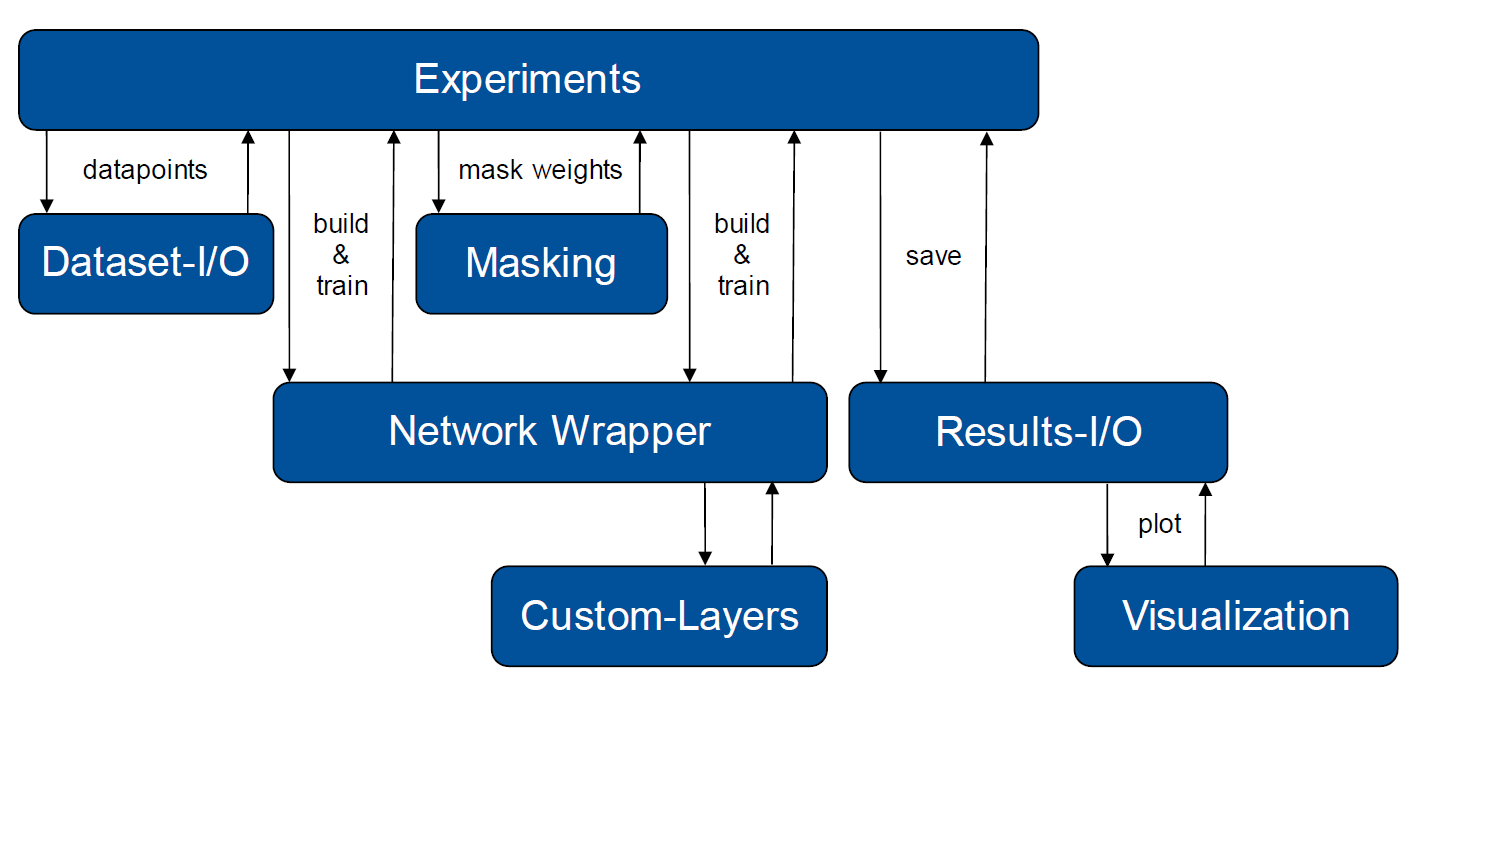
\includegraphics[width=450px]{gfx/structure.png}
	\caption{project architecture}
	\label{fig:Architecture}
\end{figure}

\section{Interaction of Components}
\begin{figure}[H]
	\centering
	\includegraphics[width=450px]{gfx/structure2.png}
	\caption{project architecture}
	\label{fig:Interaction}
\end{figure}


\section{Summary}

%*****************************************
%**************Data Sets******************
%*****************************************
%*****************************************
\chapter{Data Sets}
\label{ch:data_sets}
%*****************************************
\begin{figure}
	\begin{tabular}{c|c|c|c|c}
		& MNIST & CIFAR-10 & 20-Newsgroup & Reuters-21578\\
		\hline
		N. labels & 10 & 10 & 20 & 10 to 115\\
		N. datapoints & 70.000 & 60.000 & 18846  & 12.902\\
		fixed split & x & x & "bydate" & "ModApt\'e"\\
		shortened &  &  & x & x\\
		class imbalance &  &  &  & x\\
		multi-label &  &  &  & x\\
	\end{tabular}
\end{figure}

\section{MNIST}
The MNIST-dataset contains 25x25 gray-scale images of handwritten digits padded to 28x28 \cite{MNIST}. 

\section{CIFAR-10}

\section{20-Newsgroup}

\section{Reuters-21578}
The Reuters-21578-dataset contains 21578 articles published by the Reuters News Agency in 1987 \cite{Reuters-21578}. Reuters-21578 differs from the previous data sets in the sense that it lacks a few fundamental properties. In particular Reuters-21578 is not only multi-class but rather multi-label meaning that any one data point can satisfy multiple categories. Additionally there are categories in Reuters-21578 that have no associated positive example and even for all remaining ones the amount of samples is heavily skewed. In order to restore parts of the missing properties with minimal change to the dataset different subsets of Reuters-21578 have been chosen by different researchers.\\
F. Debole \& F. Sebastiani \cite{Reuters-Subsets} describe those subsets, starting out stating that close to half of the data points are unusable which leaves 12,902 documents. 9,603 are marked for training and 3,299 for validation.\footnote{While different training-splits were used for Reuters-21578 "ModApt\'e" has become the canonical choice} They also point out the different groups of categories used for classification:
\begin{itemize}
	\item \textbf{R$\left(115\right)$}\\
	The group with the 115 categories containing at least one positive training example.\\ 
	\item \textbf{R$\left(90\right)$}\\
	The group with the 90 categories containing at least one positive training and test example.\\ 
	\item \textbf{R$\left(10\right)$}\\
	The group with the 10 categories containing the most examples. \\
\end{itemize} 

%*****************************************
%**************Evaluation*****************
%*****************************************
%*****************************************
\chapter{Evaluation}
\label{ch:evaluation}
%*****************************************
%\hint{This chapter should describe how the evaluation of the implemented mechanism was done. \\ \\
%1. Which evaluation method is used and why? Simulations, prototype? \\
%2. What is the goal of the evaluation? Comparison? Proof of concept? \\
%3. Wich metrics are used for characterizing the performance, costs, fairness, and efficiency of the system?\\
%4. What are the parameter settings used in the evaluation and why? If possible always justify why a certain threshold has been chose for a particular parameter.  \\
%5. What is the outcome of the evaluation? \\ \\
%The section should have a length of about five to ten pages.}
The following chapter presents the results achieved throughout this thesis and aims to explain their evaluation. First, the intended goal of each experiment is stated, including a  formulation in terms of validatable benchmarks. Subsequently, the process which extracts legible data from the framework is developed. The visualized data follows, and finally, the results are analyzed.

\section{Reproduction}
\subsection*{Goal and Benchmarks}
As the latter sections evaluate explorative experiments, the validity of the framework which supports them is crucial. We trained the first two models described in sections [4] and [5] under the conditions J. Frankle and M. Corbin describe in their paper. The mismatch of weights previously described forms the only known difference.
J. Frankle and M. Corbin primarily report the accuracy achieved by their implementations at the epoch of a simple stopping criterion. They executed each experiment five times and plot the mean alongside the minimum and maximum, which are represented through error bars. Additionally, they reperformed the same experiments ten times, but applied the masks, found after each epoch, to randomly reinitialized networks. The results were visualized in the same manner. [cite LTH]
On the left side of [figure 6.1] and [figure 6.2], these measures are presented for the MNIST-FCN and the CIFAR10-CNN-6, respectively. Both plots are taken from the Lottery Ticket Hypothesis paper, but we cleaned up the latter one and brought it up to scale for improved legibility.[footnote]  The goal of this reproduction is to produce results within the reported confidence intervals of accuracy in the Lottery Ticket Hypothesis paper.  

\subsection*{Evaluation Setup}
As the produced framework does not provide any early stopping criterion, we display the full range of accuracy a given architecture achieves after convergence. A line visualizes the mean, while a gray band denotes the interval between maximal and minimal achieved accuracy. As a positive side-effect, this setup increases the breadth of visualized data in the following explorative experiments because it is parameter-agnostic concerning the early stopping criterion. Finally,  as J. Frankle and M. Corbin present training accuracies for the MNIST-Lenet-FCN architecture, we visualize the same measure for additional points of comparison.\footnote{
	For the Conv6 architecture, the effective pruning rate per iteration amalgamate its dense and convolutional pruning rate. We remind that the disagreement in the number of weights in the dense layers between our framework and the Lottery Ticket Hypothesis paper also results in a different pruning rate per epoch. 
} 
\subsection*{Evaluation Results}
As seen in figure [6.1], the MNIST-Lenet-FCN implementation we provide achieves a lower accuracy than reported by J. Frankle and M. Corbin. Additionally, it does not show an interim improvement and degrades significantly faster at advanced pruning iterations. Said degradation is qualitatively similar to the behavior of the randomly reinitialized networks.
The comparison in figure [6.2] yields similar results. While the CIFAR10-CNN-6 implementation produces the same accuracy as a full network, it degrades as quickly as J. Frankel and M. Corbin's reinitialized networks. Most of its graph falls into the deviation intervals they visualized.

\begin{figure}
	\begin{minipage}{\textwidth}
		\centering
		\includegraphics[width=100px]{gfx/7-Evaluation/LTH_3_legend.png}
	\end{minipage}
	\begin{minipage}{0.5\textwidth}
		\centering
		\includegraphics[height=180px]{gfx/7-Evaluation/LTH_0.png}
		\caption*{LTH-paper: Accuracy after convergence}
		\label{?}
	\end{minipage}\hfill
	\begin{minipage}{0.5\textwidth}
		\centering
		\includegraphics[height=180px]{gfx/Experiments/Reproduction-MNIST-FCN/accuracy/converged.png}
		\caption*{Thesis-Framework: Accuracy after convergence}
		\label{?}
	\end{minipage}
\end{figure}

\begin{figure}
	\begin{minipage}{\textwidth}
		\centering
		\includegraphics[width=100px]{gfx/7-Evaluation/LTH_4_legend.png}
	\end{minipage}
	\begin{minipage}{0.5\textwidth}
		\centering
		\includegraphics[height=180px]{gfx/7-Evaluation/LTH_CNN_clean.png}
		\caption*{LTH-paper: Accuracy after convergence}
		\label{?}
	\end{minipage}\hfill
	\begin{minipage}{0.5\textwidth}
		\centering
		\includegraphics[height=180px]{gfx/Experiments/Reproduction-CIFAR10-CNN/accuracy/LTH.png}
		\caption*{Thesis-Framework: Accuracy after convergence}
		\label{?}
	\end{minipage}
\end{figure}

\begin{figure}
	\begin{minipage}{\textwidth}
		\centering
		\includegraphics[width=100px]{gfx/7-Evaluation/LTH_1_legend.png}
	\end{minipage}
	\begin{minipage}{0.5\textwidth}
		\centering
		\includegraphics[height=180px]{gfx/7-Evaluation/LTH_1.png}
		\caption*{LTH-paper: pruned 0|3|7 times}
		\label{?}
	\end{minipage}\hfill
	\begin{minipage}{0.5\textwidth}
		\centering
		\includegraphics[height=180px]{gfx/Experiments/Reproduction-MNIST-FCN/accuracy/LTH_1.png}
		\caption*{Thesis-Framework: pruned 0|3|7 times}
		\label{?}
	\end{minipage}
\end{figure}

\begin{figure}
	\begin{minipage}{\textwidth}
		\centering
		\includegraphics[width=100px]{gfx/7-Evaluation/LTH_2_legend.png}
	\end{minipage}
	\begin{minipage}{0.5\textwidth}
		\centering
		\includegraphics[height=180px]{gfx/7-Evaluation/LTH_2.png}
		\caption*{LTH-paper: pruned 0|7|12|15|18 times}
		\label{?}
	\end{minipage}\hfill
	\begin{minipage}{0.5\textwidth}
		\centering
		\includegraphics[height=180px]{gfx/Experiments/Reproduction-MNIST-FCN/accuracy/LTH_2.png}
		\caption*{Thesis-Framework: pruned 0|7|12|15|18 times}
		\label{?}
	\end{minipage}
\end{figure}
\subsection*{Analysis of Results}
The implementations of the provided framework do not reproduce the results presented in the Lottery Ticket Hypothesis paper, meaning that the framework is not validated. This poses the question of how to proceed with the remaining experiments, which we discuss in the corresponding "Goal and Benchmarks" subsections.
While the framework did not fulfill the primary goal of the experiment, two phenomena remain unclear and intriguing:
The MNIST-Lenet-FCN architecture produces through our implementation of the Lottery Ticket algorithm degrades only by one percentage point under compression of up to ten times. Such a result is comparable to various pruning methods discussed in chapter [3]. 

%*****************************************

\section{Transfer}
\subsection*{Goal and Benchmarks}
While the reproduction experiments did not validate the framework, it still pruned the MNIST-Lenet-FCN to a degree comparable to contemporary work through, and it did so through the masking of networks with frozen initialization. As such, the transfer to another field still might yield another pruning tool for additional tasks and applications. If the framework prunes about 90 percent of weight without the sacrifice of prediction quality, we consider the transfer succesful.
\subsection*{Evaluation Setup}
While figure [6.3] presents the accuracies collected in the same manner as before, fewer pruning iterations are displayed. Due to the sheer size of the 20Newsgroups-End2End architecture and the way our framework interacts with TensorFlow 2.0 to produce pruned networks severely limited the number of pruning iterations, a single experiment could afford to run without overflowing the memory of our computing devices. We managed to run experiments with ten pruning iterations, the minimal number to prune a network to a competitive degree.
\subsection*{Evaluation Results}
The right side of figure [6.4] shows that the 20Newsgroups-End2End architecture retains its accuracy even if about 90 percent of its weights are pruned. Additionally, the networks of the intermediate pruning epochs show an accuracy improvement of at least one percentage point.
\begin{figure}
	\begin{minipage}{0.5\textwidth}
		\centering
		\includegraphics[width=100px]{gfx/7-Evaluation/20Newsgroups_legend.png}
	\end{minipage}
	\begin{minipage}{0.5\textwidth}
		\centering
		%\includegraphics[width=100px]{gfx/7-Evaluation/LTH_4_legend.png}
	\end{minipage}
	\\
	\begin{minipage}{0.5\textwidth}
		\centering
		\includegraphics[height=180px]{gfx/Experiments/Transfer-20Newsgroups-CNN/accuracy/10_iterations.png}
		\caption*{Accuracy on 20Newsgroups pruned 0-10 times}
		\label{fig:CIFAR10accuracy15}
	\end{minipage}\hfill
	\begin{minipage}{0.5\textwidth}
		\centering
		\includegraphics[height=180px]{gfx/Experiments/Transfer-20Newsgroups-CNN/accuracy/converged.png}
		\caption*{Accuracy on 20Newsgroups after convergence}
		\label{?}
	\end{minipage}
\end{figure}

\subsection*{Analysis of Results}
According to the previously defined goal, the transfer was successful, which shows that non-image-recognition architectures can contain efficient subnetworks upon initialization.

%*****************************************

\section{Early Tickets}
Independent of the ability to recover actual lottery tickets, the pruning implementation supplied by our framework finds small subnetworks in the initialization which are trainable to a nontrivial accuracy. H. Zhou et al. findings confirm that the utilization of trained weights, to calculate the pruning mask, is essential.[cite] Information on the development of the quality of said weights is still of interest. 
\subsection*{Goal and Benchmarks}
The aim of this experiment is purely explorative. If any patterns are recognized, they may inform experiments implemented with valid frameworks.
\subsection*{Evaluation Setup}
Figure [6.4] and [6.5] plot the mean accuracy achieved by implementations set to prune at the n-th epoch of training. To avoid visual clutter, the interval representing minimal and maximal values are omitted. 
\subsection*{Evaluation Results}
Because the accuracy of multiple graphs behaves erratically, it is challenging to discern a development over the training depth. The only certain observation is that all trials of earlier pruning degrade significantly faster than the original approach.
\begin{figure}
	\begin{minipage}{\textwidth}
		\centering
		\includegraphics[width=100px]{gfx/7-Evaluation/LTH_5_legend.png}
	\end{minipage}
	\begin{minipage}{0.5\textwidth}
		\centering
		\includegraphics[height=175px]{gfx/Experiments/EarlyTicket-MNIST-FCN/012.png}
		\caption*{Ticket candidates pruned at epochs 0|1|2}
		\label{?}
	\end{minipage}\hfill
	\begin{minipage}{0.5\textwidth}
		\centering
		\includegraphics[height=175px]{gfx/Experiments/EarlyTicket-MNIST-FCN/345.png}
		\caption*{Ticket candidates pruned at epochs 3|4|5}
		\label{?}
	\end{minipage}
\end{figure}
\begin{figure}
	\begin{minipage}{\textwidth}
		\centering
		\includegraphics[width=100px]{gfx/7-Evaluation/LTH_6_legend.png}
	\end{minipage}
	\begin{minipage}{0.5\textwidth}
		\centering
		\includegraphics[height=175px]{gfx/Experiments/EarlyTicket-MNIST-FCN/678.png}
		\caption*{Ticket candidates pruned at epochs 6|7|8}
		\label{?}
	\end{minipage}\hfill
	\begin{minipage}{0.5\textwidth}
		\centering
		\includegraphics[height=175px]{gfx/Experiments/EarlyTicket-MNIST-FCN/910.png}
		\caption*{Ticket candidates pruned at epochs 9 and 10}
		\label{?}
	\end{minipage}
\end{figure}
\subsection*{Analysis of Results}
While the original network converges in about ten epochs the same amount of training does not seem to suffice to achieve the full efficiency of the pruning algorithm implemented in our framework



%*****************************************
%**************Conclusions****************
%*****************************************
%*****************************************
\chapter{Conclusions}
\label{ch:closure}
%*****************************************

%\hint{This chapter should summarize the thesis and describe the main contributions of the thesis. Subsequently, it should %describe possible future work in the context of the thesis. What are limitations of the developed solutions? Which things can %be improved?
%The section should have a length of about three pages.}
To conclude this thesis, this last section summarizes the accomplished work, assures results and records possibilities for future work.

\section{Summary}
Inspired by the paper J. Frankle and M. Corbin published at the beginning of 2019, we decided to research two applications of the pruning algorithm they proposed. With the help of Tensorflow 2.0, the natural language toolkit nltk, scikit-learn, and a few additional backend applications, we developed a framework to search different architectures for lottery tickets. Afterward, we designed four experiments: two to validate the framework, one to extend this kind of pruning to new datasets, and the last one to explore the emergence of actionable training experience in an architecture.  The reproduction was not successful, but the framework still pruned the MNIST-Lenet-FCN architecture by a factor of ten while loosing less than a percentage point. The second experiment was a definite success, and the exploration of early pruning possibilities yielded no starting points for further study.

\section{Contributions}
The primary contribution of this thesis is the openly available framework we developed. While its reproduction experiments failed the, the framework achieved competitive pruning results on at least two architectures. Furthermore, the availability of source code enables any future researcher to check and rerun the tests themselves. Additionally, the success of the second experiment makes a good case for the application of the presented kind of pruning algorithm in the field of natural language processing.

\section{Future Work}
The developed framework could be a convenient tool to prune various networks, but at the moment, it is heavily limited by two factors:

Firstly, some part of the workflow fills up the working memory once per pruning iteration. Experiments with massive architectures or great pruning depth may cause a memory failure resulting in the loss of all training data. Our best guess for a cause is the Tensorflow 2.0 backend. During the restoration of weight after one training procedure has finished, it might integrate the newly pruned model into its old execution graph instead of creating a new one.

Secondly, the lack of a fourth layer of abstraction overloads the main module. As described in chapter \ref{ch:implementation}, the framework function at three such layers, but none of them should handle the control flow between and visualization. The result is an inefficient way to interface with the framework.

Finally, the success of the transfer experiment shows that the implemented pruning methodology can extend to non-image datasets. The next sensible point of order is a proof-of-concept that the method can also be extended to architectures more common in the natural language processing field, such as LSTMs.

%\section{Final Remarks}
